%%%%%%%%%%%%%%%%%%%%%%%%%%%%%%%%%%%%%%%%%
% University Assignment Title Page 
% LaTeX Template
% Version 1.0 (27/12/12)
%
% This template has been downloaded from:
% http://www.LaTeXTemplates.com
%
% Original author:
% WikiBooks (http://en.wikibooks.org/wiki/LaTeX/Title_Creation)
%
% License:
% CC BY-NC-SA 3.0 (http://creativecommons.org/licenses/by-nc-sa/3.0/)
% 
% Instructions for using this template:
% This title page is capable of being compiled as is. This is not useful for 
% including it in another document. To do this, you have two options: 
%
% 1) Copy/paste everything between \begin{document} and \end{document} 
% starting at \begin{titlepage} and paste this into another LaTeX file where you 
% want your title page.
% OR
% 2) Remove everything outside the \begin{titlepage} and \end{titlepage} and 
% move this file to the same directory as the LaTeX file you wish to add it to. 
% Then add \input{./title_page_1.tex} to your LaTeX file where you want your
% title page.
%
%%%%%%%%%%%%%%%%%%%%%%%%%%%%%%%%%%%%%%%%%
%\title{Title page with logo}
%----------------------------------------------------------------------------------------
%	PACKAGES AND OTHER DOCUMENT CONFIGURATIONS
%----------------------------------------------------------------------------------------

\documentclass[12pt]{article}
\usepackage[english]{babel}
\usepackage[utf8x]{inputenc}
\usepackage{amsmath}
\usepackage{graphicx}
\usepackage[colorinlistoftodos]{todonotes}
\usepackage{makeidx}
\usepackage[colorlinks=true,linkcolor=black,anchorcolor=black,citecolor=black,filecolor=black,menucolor=black,runcolor=black,urlcolor=blue]{hyperref}
\usepackage{color}
\usepackage{caption}
\makeindex

\begin{document}
\renewcommand\indexname{Índice}
\begin{titlepage}

\newcommand{\HRule}{\rule{\linewidth}{0.5mm}} % Defines a new command for the horizontal lines, change thickness here

\center % Center everything on the page
 
%----------------------------------------------------------------------------------------
%	HEADING SECTIONS
%----------------------------------------------------------------------------------------

\textsc{\LARGE Facultad de Informática}\\[1.5cm] % Name of your university/college
\textsc{\large Adrián García García}\\[0.5cm] % Minor heading such as course title

%----------------------------------------------------------------------------------------
%	TITLE SECTION
%----------------------------------------------------------------------------------------

\HRule \\[0.4cm]
{ \huge \bfseries Arquitecturas Cloud y microservicios}\\[0.4cm] % Title of your document
\HRule \\[1.5cm]
 
%----------------------------------------------------------------------------------------
%	AUTHOR SECTION
%----------------------------------------------------------------------------------------


% If you don't want a supervisor, uncomment the two lines below and remove the section above
%\Large \emph{Author:}\\
%John \textsc{Smith}\\[3cm] % Your name

%----------------------------------------------------------------------------------------
%	DATE SECTION
%----------------------------------------------------------------------------------------

{\large \today}\\[2cm] % Date, change the \today to a set date if you want to be precise

%----------------------------------------------------------------------------------------
%	LOGO SECTION
%----------------------------------------------------------------------------------------


\includegraphics[width=4cm,keepaspectratio]{logo.png}
 
%----------------------------------------------------------------------------------------

\vfill % Fill the rest of the page with whitespace



\captionsetup[figure]{labelformat=empty,justification=raggedright,singlelinecheck=false}
% Include image from images directory
\begin{figure}[h]

        
\includegraphics[width=2cm,keepaspectratio]{cc-by-sa.png}
        \label{fig:by-sa}
        \caption{ This work is licensed under a \href{https://creativecommons.org/licenses/by/4.0/legalcode}{CC-BY-SA 4.0 License}.}

\end{figure}

\end{titlepage}

\printindex

\begin{abstract}
Este trabajo tiene como objetivo exponer y profundizar en los conceptos expuestos en una conferencia optativa que tuvo lugar durante la semana de la informática de 2017. Los ponentes fueron dos ingenieros de la empresa GMV (Ricardo de Castro y Roberto Galán). En concreto, el nombre de la conferencia era el siguiente: Despliegue automático de arquitecturas escalables basadas en microservicios sobre el Cloud de Google (23 de Febrero, 11-14 horas). Conviene puntualizar que al final no usaron el Cloud de Google, sino que se basaron en Amazon Web Services y Docker Swarm para desplegar una aplicación web que se basaba en el uso de microservicios para su funcionamiento.
\end{abstract}

\section{Introducción}\index{Introducción}

Durante la conferencia, se hizo especial hincapié en las necesidades de los clientes y las características que estos exigen en una aplicación cloud. Los requisitos más destacados son los siguientes:

\begin{itemize}
\item \textbf{Tiempo rápido de despliegue}. Uno de los problemas más extendidos en el ámbito de las aplicaciones empresariales de elevada complejidad es que la aplicación puede tener complejas dependencias entre librerías y resulta díficil hacer un despliegue limpio y sin errores. Se ponía como ejemplo el clásico problema de que en el entorno de desarrollo funciona todo perfectamente, pero cuando se traslada a producción deja de hacerlo y cada equipo le echa la culpa a otro.
\item \textbf{Escalabilidad}. Los servicios pueden recibir grandes picos de tráfico y deben ser capaces de responder ante los mismos sin errores. Es evidente que la optimización de cada componente de la aplicación es un aspecto importante, pero además se debe diseñar un sistema capaz de balancear la carga y aumentar la dedicación de recursos replicando sus unidades de cómputo para responder ante los incrementos en demanda. Esto es relativamente fácil de hacer en entornos cloud o con soluciones de virtualización como Docker.
\item \textbf{Fiabilidad}. El funcionamiento de las aplicaciones web está íntimamente relacionado con la imágen que las grandes empresas tienen en la sociedad, si una tienda de comercio electrónico se cae durante una hora puede suponer pérdidas millonarias para la empresa y acarrea el riesgo de que sus clientes dejen de confiar en ella y pasarse a la competencia. Debido a esto, los clientes esperan que su aplicación tenga el mínimo número de errores posibles. Uno de los aspectos más importantes en este sentido es que se haga un proceso meticuloso de \emph{testing} y validación antes de publicar una aplicación, priorizando las partes más críticas del sistema y que pueden suponer un cuello de botella para la misma.
\item \textbf{Recuperación instantánea ante fallos}(\emph{Zero Down Time}). En caso de que la aplicación llegue a fallar, lo que es imposible de evitar al completo, es necesario minimizar este tiempo en el que no se provee un servicio. 
\end{itemize}


%\subsection{Subsections}\index{Section}


%\todo[inline, color=green!40]{This is an inline comment.}




% -- FIGURE --
%\begin{figure}
%\centering
%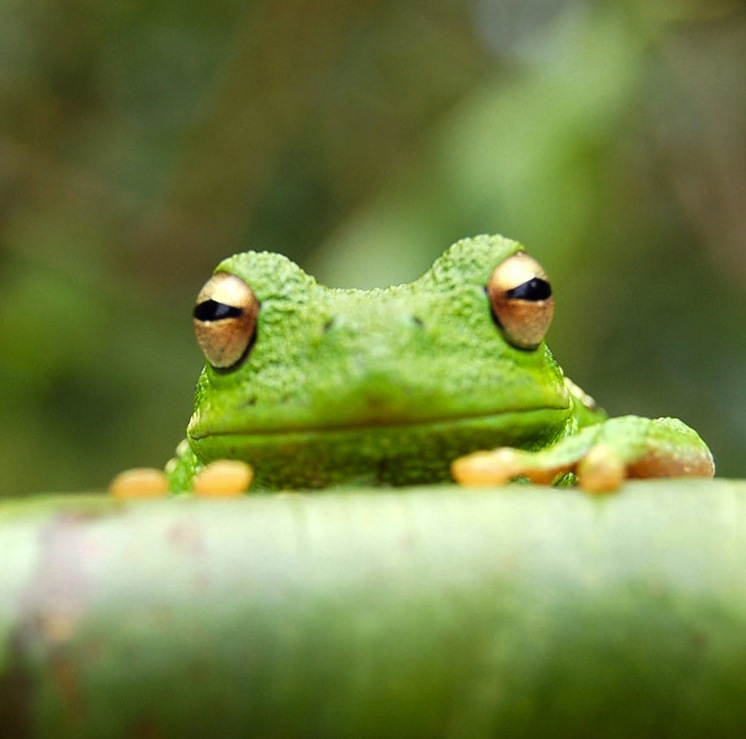
\includegraphics[width=0.5\textwidth]{frog.jpg}
%\caption{\label{fig:frog}This is a figure caption.}
%\end{figure}

% -- TABLE --
%\begin{table}
%\centering
%\begin{tabular}{l|r}
%Item & Quantity \\\hline
%Widgets & 42 \\
%Gadgets & 13
%\end{tabular}
%\caption{\label{tab:widgets}An example table.}
%\end{table}


\begin{thebibliography}{1}
%\bibitem{key} description. \href{https://...}{Enlace}
\bibitem{reliab}Fundaments of Cloud Service Reliability, Microsoft Secure Blog. \href{https://blogs.microsoft.com/microsoftsecure/2012/09/12/fundamentals-of-cloud-service-reliability/}{Enlace}.
\end{thebibliography}

\end{document}